\documentclass{hduthesis}

\setCJKmainfont{Songti SC}[AutoFakeSlant]
\setCJKsansfont{STHeiti}[AutoFakeBold = 2]
\tikzset{ > = stealth }
\usetikzlibrary{positioning,shapes.geometric}

\DocInfo
{
  title      = 杭州电子科技大学学位论文 \hologo{LaTeX} 模板/毕业论文,
  school     = 理学院,
  major      = 物理学,
  class      = 英才班,
  stdntid    = C668668E,
  author     = 申智能,
  supervisor = 李智能,
  % reference  = reference
}

\begin{document}

\maketitle

\begin{abstract}
  \hologo{hduthesis} 是杭州电子科技大学学位论文 \hologo{LaTeX} 模板,支持学士、硕士学位论文排版,同时提供了学校信笺、Slides(幻灯片)模板.
\end{abstract}

\begin{center}
  \small\bfseries 用户协议
\end{center}
\begin{enumerate} [ itemsep = 0pt ] \small
  \item 本模板通过 LPPL 1.3c 协议开放源代码,您可以随意使用编译出的 PDF 文件.
  \item 本模板根据杭州电子科技大学教务处颁发的 \href{https://jwc.hdu.edu.cn/2022/0428/c4528a153813/page.htm}{杭电理工类毕业论文写作规范} 编写而成,作者不对使用本模板产生的格式审查问题负责. \emph{如果您所在的学院因论文查重、收录等原因要求提交 \file{.docx} 格式,不接收 \file{.pdf} 论文稿件,请勿执意使用本模板,避免因格式转换带来不必要的麻烦.} 使用本模板时,请按编译错误提示操作来勾选同意用户协议.
  \item 欢迎前往 GitHub 提交反馈意见,为推动学校认证与规范化 \hologo{hduthesis} 贡献力量.
\end{enumerate}

\pagestyle{fancy}
\frontmatter
\tableofcontents
\mainmatter

\chapter{引言}

目前的射击打靶训练,基本以实弹训练为主,国防开支大,危险系数高。传统的报靶方法是人工报靶,由报靶员根据经验确定靶数,带有很大的个人主观因素,可靠性、公正性差,效率低。因此有必要研制一种切合部队实际的,在非实弹射击条件下进行射击精度训练的打靶训练器,这样既能保证部队训练质量又能减少弹药消耗、节约国防费用,具有重大的国防意义。

以光代弹,可以模拟多种武器的射击情况,并可检验射击效果。这种新型的部队训练模拟器材是部队训练器材的一次革命,是和平时期部队训练的有效手段之一。一些发达国家,如美国、英国、德国等都在积极进行激光射击模拟训练器材的研制,并已开发出多种系列产品,其中最突出的是美国的“米勒斯”系列,它可模拟 36 种武器,性能好、准确而且逼真,大大推动了部队的训练工作。

八十年代以来,我国也有单位在进行激光模拟训练器的研究和探索,将激光射击模拟器用于部队训练,取得了很好的训练效果,提高了部队的战斗力。但在可靠性和数据处理等方面尚有许多技术问题有待改进,主要是以下几点:激光光斑太大,与实际步枪子弹口径$\qty{7.62}\mm$相差太多;探测器数量少会导致设计精度不高;探测器数量多会使得价格昂贵,无法推广;只能粗略指示命中与否,不能准确显示命中靶环环数和方位。因此,我们拟从这些方向作进一步的研究探索。

本设计采用半导体激光器和半导体面阵列探测器来模拟子弹射击和射击靶标,具有模拟逼真,精度高等特点。主要从信号处理部分来设计实现激光打靶系统,每次射击能精确的显示 5 -- 10 环的结果及脱靶情况,每个环数又可分为八个偏移方向。该系统简单实用,既能保证训练的质量又能减少弹药的消耗,是理想的公安、军队等部门训练使用的模拟打靶系统。
\chapter{概述}

\section{激光打靶系统概述}

激光打靶系统\cite{cn1,cn2,cn3}的工作原理是采用激光脉冲来模拟枪弹的射击,该系统一般包括激光发射部分、激光信号检测模块、打靶成绩处理和显示部分。如图 2-1 所示,当射手瞄准完毕扣动扳机时,半导体激光器会发出激光脉冲,射向目标上的光电探测器,如果击中目标,则激光脉冲被光电探测器接收并转换为电信号,经电路处理能识别射击的弹着点,信号经处理编码后传输到计算机。

\begin{figure}[htbp]
  \centering
  \begin{tikzpicture}
  [
    every node/.style = { font = \small, inner sep = 1ex }
  ]
    \node (a) [draw, rectangle] at (0,0) {光电探测器};
    \node (b) [draw, rectangle] at (3.5,0) {信号处理电路};
    \node (c) [draw, rectangle] at (7,0) {计算机处理};
    \node (d) [draw, rectangle] at (0,-1.5) {半导体激光器};
    \node (e) [draw, rectangle] at (4,-1.5) {激光枪扳机};
    \draw [->, thick] (a.east) -- (b.west);
    \draw [->, thick] (b.east) -- (c.west);
    \draw [->, thick] (d.north) -- (a.south);
    \draw [->, thick] (e.west) -- (d.east);
  \end{tikzpicture}
  \caption{激光打靶系统原理图}
\end{figure}

半导体激光器\cite{cn4,en5}一般平行地安装在武器装备的枪管、炮管或导弹发射架上,它可以发射一束与武器射击方向一致的激光脉冲。目前的激光器一般都采用半导体激光器,因为这种激光器的输出功率低,不会伤害眼睛,而且效率高、功耗小,不但可以摆脱大而重的电源设备,激光器本身也可以制作得很小、很轻。光电探测器\cite{en6}具有射击靶的形状,可以是点探测器和面探测器,通常数量较多,构成多个信号检测通路。根据光电探测器的响应位置来判断激光射击击中的靶位。

激光打靶采用以光代弹的形式进行射击训练,是激光武器模拟器中最常见的一种。最初的激光打靶系统只能进行瞄准射击训练,随着计算机和微处理器技术的发展,其用途扩大到可进行多种武器的模拟训练。随着研究和探索的深入,激光打靶系统的功能将进一步完善,能够更接近于武器装备在实际使用中的表现,增强真实感。同时,通过与电子技术相结合,进一步提高激光模拟的自动化、智能化水平。

激光武器模拟器有以下几个方面的发展趋势:

\begin{enumerate}
  \item 可以模拟的武器越来越多,激光武器模拟器正朝着系列化、组件化的方向发展,一个基本的激光射击模拟器只要稍加改动就可适用于其他武器系统。系列化、组件化的好处是便于使用、更换和维修,同时价格也便宜。
  \item 从激光射击模拟器向激光交战模拟器发展,先进的激光交战模拟器能使坦克、战斗车辆、反坦克武器等有机的结合在一起进行训练,每部兵器既是攻击者,又是被攻击者,完全模仿实战中的作战环境,不仅能提高战士使用武器的技能,还可以教会他们如何在战争中保护自己。
  \item 采用各种新技术增加模拟的逼真性,例如用计算机来记录、控制整个训练演习的进程,评定战士在演习中的表现等。
\end{enumerate}

\section{本设计方案思路}

本设计以实现信号的良好检测和数据转换、传输为主要目的;以信号检测,信号编码和数据传输为主要设计内容。

在信号检测方面设计单脉冲小信号的放大电路和信号整形电路;在信号编码方面,要解决多路信号的编码问题,还要考虑到编码的优先选择问题;在脱靶问题的处理方法上,对打靶和信号采集传送进行同步化处理(详见第二章的硬件设计部分),把脱靶的情况与中靶的情况归为一类处理;数据传输采用 UART 串口通信。

\section{研发方向和技术关键}

\begin{enumerate}
  \item 合理划分激光靶的光电探测器,提高系统的精度;
  \item 单脉冲小信号的放大和整形;
  \item 多路优先编码器的扩展;
  \item 与微机进行数据传输,方便成绩的统计、保存、显示和查询。
\end{enumerate}

\section{主要技术指标}

\begin{enumerate}
  \item \makebox[9\ccwd][l]{激光脉宽:}大于$\qty1\ms$
  \item \makebox[9\ccwd][l]{激光脉冲响应幅度:}约$\qty{10}\mV$
  \item \makebox[9\ccwd][l]{打靶距离:}$\qty{30}\m$
  \item \makebox[9\ccwd][l]{串行输出帧格式:}射击次数\ensuremath+所击中的光电探测器的编号
\end{enumerate}
\chapter{总体设计}

激光打靶系统是一种集光、电于一体的系统,其工作原理是激光枪发出的激光束,打到光电
传感器上,经光电传感器将光信号转换为电信号,电信号经过信号处理后由单片机发送到计
算机的串行口,然后在计算机上完成成绩显示、查询和保存等功能。

激光打靶系统结构的组成框图如\cref{3-1}所示。该系统包括半导体激光枪、模块式
探测器、数字信号处理和发送电路、计算机数据处理程序等四部分。

\begin{figure}[htbp]
  \centering
  \begin{tikzpicture}
  [
    every node/.style = {font = \small, minimum height = 4.4em, minimum width = 3em}
  ]
    \linespread{1}
    \node (a) [draw, rectangle, align = center] at (0,0) {激\\光\\枪};
    \node (b) [draw, rectangle, align = center] at (2.5,0) {探测\\器\\模块};
    \node (c) [draw, rectangle, align = center] at (5,0) {滤波\\电路};
    \node (d) [draw, rectangle, align = center] at (7.5,0) {放大\\电路};
    \node (e) [draw, rectangle, align = center] at (10,0) {整形\\电路};
    \node (f) [draw, rectangle, align = center] at (12.5,0) {优先\\编码\\电路};
    \node (g) [draw, rectangle, align = center] at (2.5,-2.3) {串行\\收发\\模块};
    \node (h) [draw, rectangle, align = center] at (5,-2.3) {电平\\转换};
    \node (i) [draw, rectangle, align = center, above right] at ([yshift = -2.3cm]e.south west) {计\\算\\机};
    \draw [->, thick] (a.east) -- (b.west);
    \draw [->, thick] (b.east) -- (c.west);
    \draw [->, thick] (c.east) -- (d.west);
    \draw [->, thick] (d.east) -- (e.west);
    \draw [->, thick] (e.east) -- (f.west);
    \draw [<-, thick] (g.west) --++ (-1.5,0);
    \draw [->, thick] (g.east) -- (h.west);
    \draw [->, thick] (h.east) -- (i.west) node [midway, above = -1.5em] {串口};
  \end{tikzpicture}
  \caption{系统总体结构框图}
  \label{3-1}
\end{figure}

\section{激光的检测\cite{cn7,cn8}}

每次打靶,激光枪发出一个激光脉冲。如果激光脉冲击中光电靶,利用光生伏特效应,光电
靶上的探测器把光信号转换成电信号,因此激光的检测就是对探测器响应电信号的检测。光
电探测器的响应是一个单脉冲小信号,整个检测过程包括:信号放大、波形整形,检测输出
是标准的脉冲数字信号。

\section{靶位的划分}

把一个激光靶划分为 38 块探测器,中心 10 环为一块探测器;9.8.7.6 环分别有 8 块
探测器;5 环有 5 块探测器。根据不同靶位上的探测器来判断所击中的位置,包括环数:
10.9.8.7.6.5;偏离方向:上.下.左.右.左上.左下.右上.右下。

若信号击中两块或四块探测器的交界,则只取其中一块为有效,记为有效的探测器满足以下
条件:

\begin{enumerate}
  \item 环数高;
  \item 偏离方向为斜向(例如:上和右上两方向,选择右上)。
\end{enumerate}

根据上述要求,以及硬件电路设计的需要,对不同的探测器进行编码,见\cref{3-2}(右)。

\newpage
\begin{figure}[htbp]
  \centering
  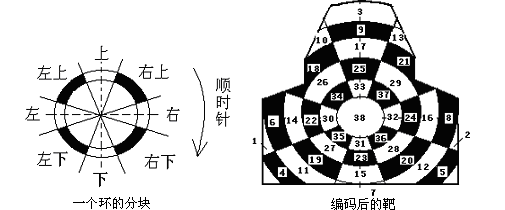
\includegraphics[width = .87\linewidth]{image-0145}
  \caption{靶位划分与编号}
  \label{3-2}
\end{figure}

\section{编码标准}

对 38 路信号按以上原则编码,编码结果如表 3-1。若脱靶无信号则记为 0 号。编码后,
每一个号码对应了每一个探测器的位置信息,包括环数和偏移方向。对信号击中两块或四块
探测器的交界的情况,只需取码号大的探测器为有效。这样,打靶的结果在硬件电路上的实现
便可由 40--6 线优先编码器完成。

\begin{table}[htbp]
  \centering
  \renewcommand{\arraystretch}{.66}
  \caption{靶位编码}
  \begin{tabular}{*{9}{@{}|@{}>{\small\centering\arraybackslash}p{.107\linewidth}}@{}|@{}}
    \hline
    & 上 & 右上 & 右 & 右下 & 下 & 左下 & 左 & 左上\\
    \hline
    10环 & \multicolumn{8}{c|}{38}\\
    \hline
    9环 & 33 & 37 & 32 & 36 & 31 & 35 & 30 & 34\\
    \hline
    8环 & 25 & 29 & 24 & 28 & 23 & 27 & 22 & 26\\
    \hline
    7环 & 17 & 21 & 16 & 20 & 15 & 19 & 14 & 18\\
    \hline
    6环 & 9 & 13 & 8 & 12 & 7 & 11 & 6 & 10\\
    \hline
    5环 & 3 & --- & 2 & 5 & --- & 4 & 1 & ---\\
    \hline
  \end{tabular}
\end{table}

\section{成绩的传送和处理}

信号经编码后发送到计算机,由计算机进行译码,在计算机上模拟显示出射击位置,对一组
结果进行统计(包括环数和方向偏移),并进行储存。

\section{其他说明}

系统分为硬件部分和软件部分。本论文主要设计制作硬件部分以及与微机的通讯的 2051 单
片机程序。微机软件部分,包括数据的处理和显示等有另外一名毕业设计同学实现。

\printbibliography
\chapter{硬件设计}

\section{信号放大电路}

在光电探测系统中,探测器输出的电信号非常微弱,一般为毫伏级。为记录每一次打靶的结果,信号放大与处理电路是打靶系统中不可或缺的。在探测器上直接进行信号处理十分困
难,一种常用的解决办法是在探测器后接前置放大器,用来放大探测器的输出信号,然后成
功地传输到信号处理系统的有关电路部分。前置放大器的设计要求是低噪声,高增益,低输
出阻抗,大的动态范围,和较好的抗噪声能力。

在激光打靶系统中,对光电池产生的脉冲信号的具体大小值要求不高,只需检测出有效的脉
冲信号,因此可选用集成运放来组成运算放大电路。

通过测试,得到光电探测器对的激光脉冲的响应幅度典型值约为$\qty5\mV$,若激光击中
在两块或多块探测器边界处,则任何一块光电探测器的响应幅度会减少,因此所检测的脉冲
幅度范围大约是$\num3\sim\qty5\mV$.为使每块光电探测器均能检测出信号,使之达到
TTL 电平要求,实现信号检测,必须对信号放大约 1000 倍。单级运放难以达到这么高的
放大倍数,因此采用二级运放进行放大,第一级为前置放大器。为减少前级放大器的偏移对
后级放大器的影响,设计其放大倍数$A_1=100$;从而次级放大器的放大倍数$A_2=10$。

\subsection{集成运算放大器(LM324)}

集成运算放大器是实现高增益放大功能的一种集成器件\cite{cn9},早期主要用来实现对模拟量进行
数学运算的功能,目前随着器件性能的改进,它已成为通用的增益器件,应用范围非常广泛。

从电特性来看,集成运放接近理想的电压放大器件,它不仅有很大的输入电阻和很小的输出
电阻,而且还有很高的电压增益,此外,静态工作时,它的输入和输出电位均为零,这样,
在与其它集成运放连接时,就不需要考虑它们之间的电平配置问题。

LM324 是四通道的低功耗运算放大器,它的内部包含四组形式完全相同的运算放大器,除电
源共用外,四组运放相互独立,其性能参数有以下几个方面:

\begin{enumerate}
  \item 单电源工作方式,工作电平$\qty3\V\sim\qty{30}\V$
  \item 低消耗电流:约$\qty{0.8}\mA$
  \item 低输入偏移:输入电压偏移:$\qty3\mV$(Typ);输入电流偏移:$\qty2\nA$(Typ)
  \item 开环增益:$\qty{100}\V/\unit\mV=\qty{100}\dB$(Typ)
  \item 宽响应频带
\end{enumerate}

\newpage
\begin{figure}[htbp]
  \centering
  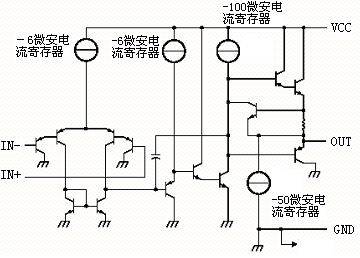
\includegraphics[width = .595\linewidth]{image-0162}
  \caption{LM324内部结构}
  \label{4-1}
\end{figure}

\subsection{放大电路图}

\begin{figure}[htbp]
  \centering
  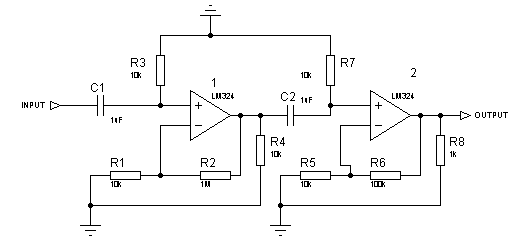
\includegraphics[width = .93\linewidth]{image-0163}
  \caption{运算放大器电路图}
  \label{4-2}
\end{figure}

放大器电路如\cref{4-2} 所示。它由两级结构相同的同相放大器组成,集成放大器选用
LM324(\cref{4-1})。信号经隔直流电容C1从第一级放大器的正端
``\ensuremath+''输入,经过放大后输出,再经过级间耦合电容C2输入第二级放大器
的正端。前级的放大倍数$A_1=R_2/R_1=100$,后级的放大倍数$A_2=R_6/R_5=10$,
$R_3$和$R_7$为输入匹配电阻。

\subsection{电路原理}

\begin{enumerate}
  \item 同相放大器\cite{cn10}(\cref{4-3})
  
  集成运放是一种十分理想的增益器件,性能好,使用方便。该电路采用 2 级放大器级
  联,每级的放大器均采用同相放大。

  由集成运放构成的同相放大器,其特点是输入信号加在同相输入端,而反馈信号加在反相端。根据理想化条件,由于$v_+=v_s$,因而$v_-\approx v_s$。更具$i\to0$(虚断),$v_-$又是$v_o$在$R_1$上的分压值,即:
  \begin{equation}
    v_-=v_o\frac{R_1}{R_1+R_f}
  \end{equation}
  因而,放大器的增益:
  
  \begin{equation}
    A_{Vf}=\frac{v_o}{v_s}=\frac{R_1+R_f}{R_1}=1+\frac{R_f}{R_1}
  \end{equation}
  $\because A_{Vf}>0$,所以$v_o$与$v_s$同相。
  
  \begin{figure}[htbp]
    \centering
    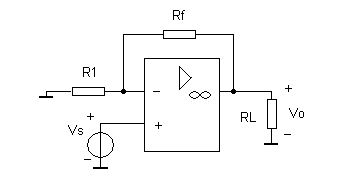
\includegraphics[width = .54\linewidth]{image-0236}
    \caption{同相放大器}
    \label{4-3}
  \end{figure}
  \item 外围电路
  
  光电传感器对外部光线也有响应,因此必须滤除这种干扰。由于背景光线是持续信号,其
  响应主要是直流量,在第一级放大器输入端的前面设计接入一个$\qty1\uF$电容C1起到
  隔离直流作用,能起到很好的效果。第二级的$\qty1\uF$电容C2用于两级放大器的耦合。

  第一级放大器输入端和地之间接 R3;第二级放大器输入端和地之间接 R7。使得:
  \begin{equation}
    \begin{cases}
      R_3\approx R_1//R_2\\
      R_7\approx R_5//R_6
    \end{cases}
  \end{equation}
  这样,运放的正、负输入端对地的等效电阻相等,从而降低运放的电压偏移。
\end{enumerate}

\subsection{电路参数}

\begin{enumerate}
  \item \makebox[9em][l]{输入脉冲幅度:} $U_i\approx\num3\sim\qty5\mV$
  \item \makebox[9em][l]{输入电阻:} $R_i\approx\qty{10}\kohm$
  \item \makebox[9em][l]{输出电阻:} $R_o\approx\qty1\kohm$
  \item \makebox[9em][l]{放大倍数:} $A=A_1\cdot A_2\approx10\times100=1000$
  \item \makebox[9em][l]{放大器级数:} 两级,前级$A_1\approx100$;后级$A_2\approx10$
  \item \makebox[9em][l]{耦合方法:} 电容耦合
\end{enumerate}

\clearpage
\vspace*{-1.5em}
\section{整形电路\cite{cn11}}

光电池的输出脉冲并不是规则的矩形脉冲信号,而是类似升余弦信号。再经放大后也会产生
失真,因此必须对信号进行整形。采用常用的 CD4093 施密特触发器便可实现整形功能,改
善脉冲波形,确保后续编码器的正常编码。

施密特触发器不仅可以进行波形整形,它的迟滞特性还可以有效地克服噪声和干扰的影响,只要噪声和干扰的大小处在迟滞宽度内,就不会有错误的输出。施密特触发器属于电平触
发,对于缓慢变化的信号仍然适用,当输入信号达到阈值电压时,电路状态发生转换,通过
电路内部的正反馈过程使得输出电压的波形的边沿变得很陡峭。利用施密特触发器可以实现
有效脉冲的识别见\cref{4-5}。

\begin{figure}[htbp]
  \centering
  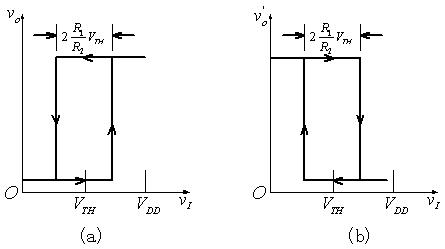
\includegraphics[width = .65\linewidth]{image-0284}
  \caption{施密特触发器的电压传输特性 (a) 同相输出;(b) 反相输出}
  \label{4-4}
\end{figure}

\begin{figure}[htbp]
  \centering
  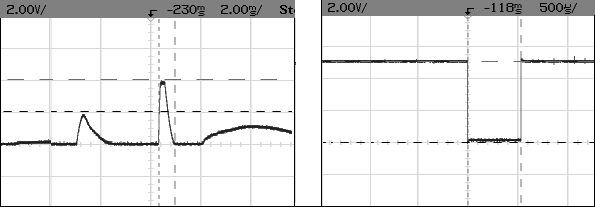
\includegraphics[width = .95\linewidth]{image-0285}
  \caption{利用施密特触发器实现有效脉冲的识别}
  \label{4-5}
\end{figure}

\section{编码电路\cite{cn11}}

对于 38 路信号通道,必须对其进行编码以便于信号识别和传输。38 路信号按照设计方案
编码为 1--38 号,脱靶无信号记为 0 号。对多个探测器同时接收到信号的情况,对应于
探测器的码号就是取码号大的探测器为有效,采用优先编码器便可实现编码的优先选择。

商用的单个优先编码器的编码输入最多只有 8 路,要构成更多路的优先编码
器,可以采用 6 片 8-3 优先编码器进行扩展为 40-6 优先编码器。

\subsection{编码电路图}

\begin{figure}[htbp]
  \centering
  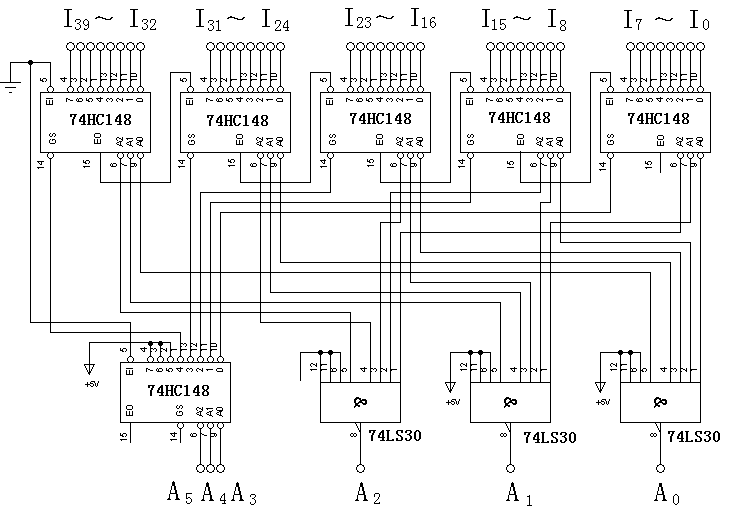
\includegraphics[width = .96\linewidth]{image-0289}
  \caption{40-6 优先编码器电路图}
  \label{4-6}
\end{figure}

\subsection{电路原理}

\begin{enumerate}
  \item 优先编码器(74HC148)
  
  8-3 线优先编码器的功能表如\cref{4-7}。待编码的 8 条输入线 采用 8 中取 1 
  码,逻辑 0 有效,编码后的输出 用反码表示。可以看出,编码器是以输入为 0 的最高
  优先编码的,而低位若同时输入 0,则是无意义的。此外,电路还设有选通输入,即使能
  端 EI,它也是逻辑 0 有效;输出还设有允许输出端 Eo 及允许扩展端 Gs,利用它们
  可判断出 是否有效,以及是否允许扩展编码。根据真值表,写出编码器的逻辑表达式如下:
  \begin{equation}
    \begin{aligned}
      \overline{A_2}&=\overline{EI}\cdot I_7+\overline{EI}\cdot I_7\cdot I_6\cdot\overline{I_5}+\overline{EI}\cdot I_7\cdot I_6\cdot I_5\cdot\overline{I_4}\\
      &=\overline{EI}(\overline{I_7}+I_7\overline{I_6}+I_7I_6I_5\overline{I_4})=\overline{EI}(\overline{I_7}+\overline{I_6}+\overline{I_5}+\overline{I_4})
    \end{aligned}
  \end{equation}
  故:
  \begin{equation}
    A_2=\overline{\overline{EI}(\overline{I_7}+\overline{I_6}+\overline{I_5}+\overline{I_4})}
  \end{equation}
  同理:
  \begin{gather}
    A_1=\overline{\overline{EI}(\overline{I_7}+\overline{I_6}+I_5I_4\overline{I_3}+I_5I_4I_2)}\\
    A_0=\overline{\overline{EI}(\overline{I_7}+I_6\overline{I_5}+I_6I_4\overline{I_3}+I_6I_4I_2\overline{I_1})}
  \end{gather}
  而允许输出为:
  \begin{equation}
    E_OE_0=\overline{\overline{EI}\cdot I_7I_6I_5I_4I_3I_2I_1I_0}
  \end{equation}
  允许扩展端是:
  \begin{equation}
    Gs=EI+\overline{EI}\cdot I_7\;I_6\;I_5\;I_4\;I_3\;I_2\;I_1\;I_0=\overline{\overline{EI}\cdot E_O}
  \end{equation}

  \begin{table}[htbp]
    \centering\scriptsize
    \renewcommand\arraystretch{1.12}
    \begin{tabular}{|>{\centering\arraybackslash\sffamily}p{.04\linewidth}|*{8}{>{\centering\arraybackslash\sffamily}p{.04\linewidth}}|*{3}{>{\centering\arraybackslash\sffamily}p{.04\linewidth}}|*{2}{>{\centering\arraybackslash\sffamily}p{.04\linewidth}}|}
      \hline
      \multicolumn{9}{|>{\sffamily\bfseries}c|}{INPUTS} & \multicolumn{5}{>{\sffamily\bfseries}c|}{OUTPUTS}\\
      \hline
      EI & 0 & 1 & 2 & 3 & 4 & 5 & 6 & 7 & A2 & A1 & A0 & GS & EO\\
      \hline
      H & X & X & X & X & X & X & X & X & H & H & H & H & H\\
      L & H & H & H & H & H & H & H & H & H & H & H & H & L\\
      L & X & X & X & X & X & X & X & L & L & L & L & L & H\\
      L & X & X & X & X & X & X & L & H & L & L & H & L & H\\
      L & X & X & X & X & X & L & H & H & L & H & L & L & H\\
      L & X & X & X & X & L & H & H & H & L & H & H & L & H\\
      L & X & X & X & L & H & H & H & H & X & L & L & L & H\\
      L & X & X & L & H & H & H & H & H & X & L & H & L & H\\
      L & X & L & H & H & H & H & H & H & X & H & L & L & H\\
      L & L & H & H & H & H & H & H & H & X & H & H & L & H\\
      \hline
    \end{tabular}
    \caption{8-3 线优先编码器真值表(74HC148)}
    \label{4-7}
  \end{table}
  \item 8-3 线优先编码器扩展为 40-6 线优先编码器(\cref{4-6})
  
  5 片 74HC148 并排用作输入,其输入从低位片到高位片排列为
  $I_0\sim I_{39}$ 。每一个高位片的输出允许端 Eo 接其相对低位片的使能端 EI。这样,当总使能$\text{EI}=0$时,允许电路进行编码工作,若高位片的诸输入中有一
  个为$0$时,该片的 $\text{Eo}=1$,$\text{Gs}=0$,这样就禁止了低位片的编
  码,以此类推,5 片 74HC148 的输入端编码便具有了优先性。

  5 片 74HC148 的允许扩展端 Gs 按低位片至高位片的顺序分别接到第六片74HC148
  的$I_0$、$I_1$、$I_2$、$I_3$、$I_4$输入端,而$I_5$、$I_6$、$I_7$端则接
  高电平(表示无输入)。这样第六片 74HC148 的三位输出便表示整个 40-6 线优先编
  码器的高三位$A_5$、$A_4$、$A_3$。而 40-6 线优先编码器的低三位输出$A_2$、$A_1$、$A_0$与前 5 片 74HC148 的输出端一致。

  由于 74HC148 的输出端不是三态门,不能直接连接在一起。而把 5 片 74HC148的同
  名输出端接到 74LS30(8 输入的与非门)取与非便可以解决这个问题。同时输出取反,
  输出为逻辑 1 有效。为使高三位输出与低三位输出一致,用 CD4049反相器对高三位取
  反。
  
  40-6 线优先编码器的六个输出均为逻辑 1 有效,可以接到后续的 2051 单片机进行串
  行传输。
\end{enumerate}

\section{串行传送}

为实现将编码器输出的 6 位并行信号串行传送,同时实现数据发送和打靶射击的同步性。采
用 89C2051 单片机便可实现要求。

\subsection{单片机及外围电路图}

\begin{figure}[htbp]
  \centering
  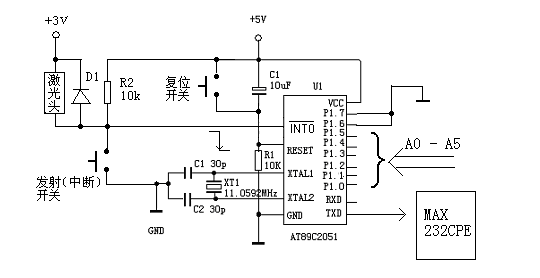
\includegraphics[width = .86\linewidth]{image-0419}
  \caption{2051 单片机及其外围电路图}\label{4-8}
\end{figure}

\subsection{电路原理}

\begin{enumerate}
  \item 编码器的输出通过 2051 P1 口的低 6 位(高 2 位接地为逻辑 0)输入。
  \item 选用 $\qty{11.0592}\MHz$ 的晶振构成单片机的时钟,这样在串口工作方式 1 下可得到准确的 $\qty{9600}{bps}$ 的串行波特率,方便计算机的接收。
  \item 单片机接有复位开关按钮。
  \item 实现打靶和信号采集传送的同步化。
\end{enumerate}

由于采用单片机的外部中断 0($\overline{INTO}$)作为数据串行传送的使能端,且
$\overline{INTO}$设为下降的跳变沿有效。使能开关(激光枪的开关)一端接地,另一
端接$\overline{INTO}$,又经上拉电阻接到电源,这样当开关按下时,便有下降沿的跳变信号输入$\overline{INTO}$,产生中断。

同时,开关又要同步控制激光枪的发射。因此开关又接激光头的负端,从而控制激光头负端
的接地,只有当开关按下时,激光头两端才有工作电压。

这样,同一个开关既控制单片机的中断,又同时控制激光枪的发射,从而达到打靶和信号采
集传送这两个“动作”的同步化。

\subsection{AT89C2051 单片机\cite{cn12}}

AT89C2051 单片机是 AT89C51 的简化型号,其指令系统和内部 RAM 均与 AT89C51相
同。不同的是它的内部 ROM 为 2k,而 89C51 为 4k,而且 2051 比 89C51 少了 P0
和 P2 输入/输出口以及外部 ROM、RAM 的扩展端,因此在引脚上 2051 只有 20 个脚。
AT89C2051 单片机主要适用于较为简单的微控制系统。在本系统中,用到 AT89C2051的 
6 个外部 I/O 口,一个外部中断和串行输出口。

\newpage
\begin{figure}[htbp]
  \centering
  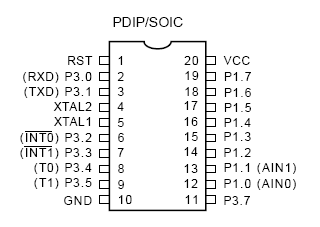
\includegraphics[width = .53\linewidth]{image-0439}
  \caption{2051 信号引脚图}
  \label{4-9}
\end{figure}

\section{电平转换}

在不同的数字系统中,其电平标准是不同的。该系统中就包括了 TTL 电平标准和 RS-232 
电平标准,要实现两个标准的正常通信,必须进行电平转换。该系统采用使用简单的 
MAX232CPE 芯片。

一片MAX232CPE芯片可完成2路TTL/CMOS~RS-23 的电平转换和2路RS-232~TTL/CMOS
的电平转换。实际电路中只有一路单片机的 TXD 串口输出,不进行RXD串口输入。因此,选
用引脚 11 接 2051 TXD 串口输出;而对应的 14 脚则接到计算机的串口输入端。

\begin{figure}[htbp]
  \centering
  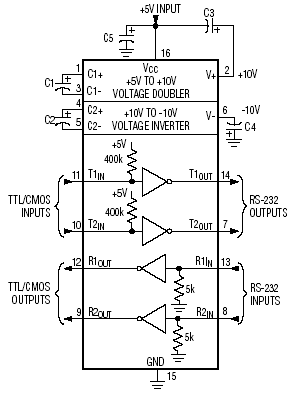
\includegraphics[width = .52\linewidth]{image-0440}
  \caption{MAX232CPE 芯片内部结构}
  \label{4-10}
\end{figure}
\chapter{软件设计}

\section{总体方案}

该系统的信号检测与数据传送部分,涉及的软件部分较少。主要是 2051 单片机数据串行通
信及通信协议的程序设计。

对于 2051 的程序设计\cite{cn12},由于所需实现的功能较简单,采用汇编的形式。编
译器采用 Keil 7.02b。该编译器是 51 系列单片机程序设计的常用工具,既可用汇编,
也支持 C 语言编译。同时具有完善的调试功能。

\section{程序流图}

\begin{figure}[htbp]
  \centering
  \begin{tikzpicture}
  [
    every node/.style = { font = {\small}, minimum height = 3em}
  ]
    \node [draw, rectangle, minimum width = 12em, minimum height = 2em] (a) at (0,0) {初始参数设置};
    \node [draw, rectangle, minimum width = 10em, rounded corners = 1.2em, below = of a] (b) {等待中断};
    \node [draw, rectangle, minimum width = 11em, diamond, aspect=3, below = of b] (c) {中断服务程};
    \node [draw, rectangle, minimum width = 11em, diamond, aspect=3, below = of c, yshift = 2ex] (d) {读取 P1 口值};
    \node [draw, rectangle, minimum width = 8em, rectangle, below = of d, minimum height = 2em] (e) {发送数据帧};
    \node [draw, rectangle, minimum width = 11em, diamond, aspect=3, below = of e] (f) {延时$\qty{200}\ms$};
    \node [draw, rectangle, minimum width = 8em, rectangle, below = of f, minimum height = 2em, yshift = 2ex] (g) {清中断标志};
    \node [draw, rectangle, minimum width = 10em, rounded corners = 1.2em, below = of g] (h) {中断返回};
    \draw [->] (a.south) -- (b.north);
    \draw [->] (b.south) -- (c.north);
    \draw [->] (c.south) -- (d.north);
    \draw [->] (d.south) -- (e.north);
    \draw [->] (e.south) -- (f.north);
    \draw [->] (f.south) -- (g.north);
    \draw [->] (g.south) -- (h.north);
    \draw [->] (h.east) --++ (1,0) |- (b.east);
  \end{tikzpicture}
  \caption{串行发送流程图}
  \label{5-1}
\end{figure}

\vspace*{-1.5em}
\section{模块说明}

\begin{enumerate}
  \item 主程序:
  \begin{lstlisting}[basicstyle=\linespread{1.32}\small\ttfamily\selectfont, breaklines=true]
      MAIN:
      MOV SP,#0X60  ;堆栈初始化
      CALL INIT     ;各寄存器参数设置
      MOV 40H,#0x01 ;打靶次数置 1
      AJMP $        ;等待中断
  \end{lstlisting}
  \item 初始化程序:
  \begin{lstlisting}[basicstyle=\linespread{1.32}\small\ttfamily\selectfont, breaklines=true]
      INIT:
      MOV TMOD,#0X21;波特率发生器
      MOV TL1,#0XFD ;波特率 9600bps
      MOV TH1,#0XFD
      CLR ET1       ;禁止 timer1
      SETB PT1      ;时钟 1 优先级:高
      MOV SCON,#0x40;串口工作模式 1,SM2=0,REN=0
      MOV PCON,#0   ;波特率 9600bps
      SETB EA       ;中断允许
      CLR PS        ;关闭串口中断
      CLR ES        ;串口优先级:低
      SETB EX0      ;开外部中断 INT0 SETB IT0 ;下降沿有效
      CLR PX0       ;INT0 优先级:低
      SETB TR1      ;时钟 1 开始计数
      RET
  \end{lstlisting}
  \item 中断服务程序:
  \begin{lstlisting}[basicstyle=\linespread{1.32}\small\ttfamily\selectfont, breaklines=true]
      _INT0:        ;ISR 中断服务程序
      NOP
      CALL DELAY_2MS;同步延时
      MOV P1,#0xff  ;读 P1 口前先置 1
      MOV A,P1      ;读 P1 口
      CALL INT0_SEND
      RET
  \end{lstlisting}
  \item 数据帧传送子程序:
  \begin{figure}[htbp]
    \centering\small
    \setstretch{1.4}
    \caption{数据帧格式}
    \begin{tabular}{|*{4}{>{\centering\arraybackslash}p{.22\linewidth}|}}
      \hline
      标志位SYNC & 打靶次数 & 打靶成绩 & 校验位CHECKSUM\\
      \hline
      \#0x30 & TIMES & RESULT & TIMES\ensuremath+RES\\
      \hline
    \end{tabular}
  \end{figure}
  \clearpage
  例:30 02 15 17(十六进制)
  
  表示第二次打靶,击中第 21 号(对应环数:7 环 偏移方向:右上)。
  \begin{lstlisting}[basicstyle=\linespread{1.32}\small\ttfamily\selectfont, breaklines=true]
      INT0_SEND:      ;数据帧传送子程序
      PUSH ACC        ;保护 ACC
      CLR A
      ADD A,#0X30
      CALL UART_SEND  ;发送标志位
      MOV A,40H
      CALL UART_SEND  ;发送打靶次数
      POP ACC
      CALL UART_SEND  ;发送打靶成绩
      ADD A,#0X30
      ADD A,0040H
      CALL UART_SEND  ;发送校验位
      INC 0040H       ;打靶次数累加 1
      CALL DELAY_200MS;延时 200ms
      CLR EX0         ;关外部中断
      CLR IE0         ;清INT0外部中断请求标志位—防止外部中断寄存
                        而引起多次中断。
      SETB EX0        ;开中断
      RETI
  \end{lstlisting}
  \item 串行发送字节
  \begin{lstlisting}[basicstyle=\linespread{1.32}\small\ttfamily\selectfont, breaklines=true]
      UART_SEND:      ;串行发送一个字节
      MOV SBUF,A
      JNB TI,$        ;等待发送完毕
      CLR TI          ;
      RET
  \end{lstlisting}
  \item 定时程序:
  \begin{lstlisting}[basicstyle=\linespread{1.32}\small\ttfamily\selectfont, breaklines=true]
      DELAY_2MS:      ;用定时器延时 2ms
      MOV R7,#21;21
      DLY1:MOV R6,#42
      DLY2:DJNZ R6,DLY2
      DJNZ R7,DLY1
      RET
      DELAY_10MS:     ;调用 DELAY_2MS,实现延时 10ms
      MOV R5,#5
      DLY: CALL DELAY_2MS
      DJNZ R5,DLY
      RET
\end{lstlisting}
\end{enumerate}
\chapter{制作与调试}

\section{硬件电路的布线与焊接}

\subsection{总体特点}

该系统所涉及的各部分硬件电路,总体的特点是:

\begin{enumerate}
  \item 电路原理简单,所用的器件均为常用器件。
  \item 由于路数较多(38 路),电路的规模较大,因此在制作中只做了 8 路。因此,
  应合理布线,以降低焊接难度,降低出错率,同时防止干扰。
\end{enumerate}

\subsection{电路划分}

为方便焊接与调试,把电路划分为两大块:

\begin{enumerate}
  \item 探测器接收,放大电路和整形电路为一块电路板;
  \item 编码器、2051 单片机和控制开关为一块电路板。
\end{enumerate}

\subsection{焊接}

焊接前应熟悉各芯片的引脚,焊接时参照电路图,仔细地连接引脚。按照以
下原则进行焊接:

\begin{enumerate}
  \item 先焊接各芯片的电源线和地线,这样确保各芯片有正确的工作电压;
  \item 同类的芯片应顺序焊接,在一片焊接并检查好之后,其他的同类芯片便可以参照第
  一片进行焊接。这样便可大大节省时间,也可降低出错率。
\end{enumerate}

\section{调试}

\begin{enumerate}
  \item 在 40-6 线优先编码器,由于没有详细阅读优先编码器的真值表,我认
  为优先编码器为低位优先,因此所设计的编码标准(取小号有效)不符合标准。
  不过发现错误后,对硬件电路无需修改,只要修改编码标准为取大号有效,便可
  以解决问题。
  \item 由于光电池的响应信号经放大、编码,到达单片机 P1 口时有一定的延
  时,为使单片机准确地通过外部中断进行有效数据的采集,应知道延时的大概范
  围。编写单片机程序时,编写了一个延时 2ms 的子程序,可以调用进行一定的延
  时,通过延时时间不同的程序进行多次烧录并进行调试,然后比较所得的不同结
  果,这样便可以大概知道要采集正确的数所需的延时时间(最后程序采用的延时
  时间为$\qty2\ms$)。
  \item 电路中同时控制激光发射和单片机外部中断的开关为普通的按钮开关,
  因此在按下和弹起都有颤动,这样会引起单片机外部中断的多次响应,使一次``射
  击动作''引起多次响应,单片机输出多个值。通常的消颤方法有两种:硬消颤和
  软消颤。硬消颤指通过硬件上的消颤电路使开关的一次动作只能产生一个脉冲跳
  变;而软消颤主要通过延时或对响应的屏蔽来实现。在该设计中采用较为简便的
  软消颤,具体的方案见第五章。
\end{enumerate}
\chapter{结论}

本设计方案达到了任务书的要求,实现了激光信号的检测、编码和串行传输,实现了较为完整的激光打靶系统的信号处理:
\begin{enumerate}
  \item 前端放大器的放大倍数适中,放大后,有效电压脉冲的幅度达到施密特触发器的上门限电压,背景干扰信号没有引起电路的误响应;
  \item 经过调试,实现 40-6 优先编码器的扩展,编码值输出符合真值表,编码有效脉冲下降沿的波形正常;
  \item 由开关按钮(模拟激光枪的扳机)控制的编码采集和串行传送也调试实现(通过与计算机的串口相连,用``串口调试程序''调试);
  \item 信号处理电路通过串口连接到计算机,应用张雪荣同学设计的``激光打靶成绩统计''软件进行总体调试,实现对打靶成绩的显示统计和储存。
\end{enumerate}

由于时间、水平和经验有限,在信号的放大、编码及抗干扰等方面仍有不足之处,有改进的余地,比如电路规模的精简,其他的光干扰处理。另外在系统的调试方面,由于时间和设备的原因,只进行了短距离的调试,有待进一步的调试。这次毕业设计对于我来说,既是一次机遇,又是一次挑战。通过这次的毕业设计,我学到了很多东西,通过自己的实践,增强了动手能力。通过实际工程的设计也使我了解到书本知识和实际应用的差别。在实际应用中遇到很多的问题,这都需要我对问题进行具体的分析,并一步一步地去解决它。
\chapter*{致谢}

在这几个月的时间里,从对课题的理解,方案的设计,到电路的制作,再到论文的写作,中
间有着自己的努力,更有着老师和同学的关心和巨大的帮助。

感谢秦会斌老师在很忙的情况下,为我讲解课题的要点,引领设计的思路。他对学生认真负
责的态度让我由衷地敬佩。

感谢唐大勇和章国平同学给予我无私的帮助,他们对我所遇到的难题的解答让我受益匪浅。

感谢罗老师对我们的关心照顾。

感谢母校和老师们在大学四年中对我的培养。

......
\printbibliography

\appendix
\chapter*{附录}

\end{document}
